\documentclass[11pt,a4paper]{article}
\usepackage[margin=2.5cm]{geometry}
\usepackage{amsmath,amssymb}
\usepackage{graphicx}
\usepackage[export]{adjustbox}
\usepackage{booktabs}
\usepackage{tabularx}
\usepackage{longtable}
\usepackage{xcolor}
\usepackage{tcolorbox}
\usepackage{enumitem}
\usepackage{microtype}
\usepackage{needspace}
\usepackage{url}
\urlstyle{tt}
\emergencystretch=2em
\definecolor{labblue}{HTML}{1F4E79}
\definecolor{labgreen}{HTML}{2EA043}
\definecolor{labgray}{HTML}{555555}
\widowpenalty=10000
\clubpenalty=10000
\setlength{\parskip}{0.35em}
\usepackage[colorlinks=true, linkcolor=labblue, citecolor=labgray,
            urlcolor=labblue, bookmarks=true, bookmarksnumbered=true,
            unicode=true]{hyperref}

\hypersetup{
    pdftitle={Klein Tunneling in Real Time: Supertansmission Against a Schrödinger Control},
    pdfauthor={Isaev, Iskhak Khamzatovich},
    pdfsubject={AB-Cloud Dirac Laboratory — per-test monograph D5},
    pdfkeywords={Dirac equation, Hofstadter model, Riemann zeta zeros, AB-Cloud, D5}
}
\begin{document}

\noindent{\small\color{labgray}\texttt{AB-Cloud Dirac Laboratory · per-test monograph · D5 · seed 96 · v1.4}}\\[0.3em]
\rule{\textwidth}{0.8pt}\\[0.6em]
{\LARGE\bfseries\color{labblue} Klein Tunneling in Real Time: Supertansmission Against a Schrödinger Control}\\[0.5em]
{\normalsize\itshape Test D5 — $T(0°) = 0.9777$ vs $0.0010$: a factor of 977, watched frame by frame}\\[0.4em]
\rule{\textwidth}{0.4pt}

\begin{tcolorbox}[colback=labgreen!8, colframe=labgreen!70!black, title={Verdict: PASS — 4/4 checks}, fonttitle=\bfseries, boxrule=0.6pt]
\textbf{Abstract.} Test D5 verifies the most famous paradox of the Dirac equation by real-time numerics: a massless Dirac wave packet crosses a potential barrier that is classically forbidden -- and that perfectly traps a Schrödinger packet -- with transmission $T(0°) = 0.9777$ against $0.0010$ for the Schrödinger control, a factor of 977 under identical geometry \cite{klein}. The angular law collapses as measured: $T(60°)/T(0°) = 0.005$, the chiral-suppression signature of pseudospin mismatch. The simulation is an exact spectral propagation on a finite grid with no absorbing boundaries inside the measurement window.
\end{tcolorbox}

\section{What This Test Verifies}
Klein tunneling is the counter-intuitive consequence of the Dirac equation's two-band structure: inside a strong potential the negative-energy sea supplies propagating states, so a normally incident massless Dirac particle cannot be reflected at all -- $T(0°) = 1$ in the continuum idealization \cite{klein,dirac}. A Schrödinger particle meeting the same barrier is exponentially suppressed. The effect is angularly fragile: at oblique incidence the pseudospin mismatch between the two sides restores reflection, and $T(\theta)$ collapses on the scale set by the barrier momentum.

Within the AB-Cloud programme this test has a specific operational value. The vortex phases of the parent construction are, from the electron's viewpoint, a landscape of strong local gauge fields; whether packets survive such a landscape -- whether the substrate is a resonator or a wall -- is precisely a Klein-tunneling question. D5 answers it in the clean limit and calibrates the real-time machinery that D10 and D11 will reuse for the $\zeta$-decorated transport tests \cite{parent}.

\section{Model and Method}
A Gaussian wave packet ($k_0 = 0.45$, minimal width) is launched at a smooth barrier on a periodic grid; the Dirac channel uses the laboratory's Hermitian symmetric-difference momentum $p_d = -i(S^+ - S^-)/(2dx)$, and the Schrödinger channel uses the matching $-\frac{1}{2}\nabla^2$ discretization. Both are propagated by exact spectral evolution ($e^{-iHt}$ via dense eigen-decomposition of the modest grid), so there is no time-stepping error and no absorbing boundary inside the window. Transmission is measured as the integrated probability beyond the barrier after the packet has fully cleared it, with the reflection-side residue cross-checked.

The angle scan repeats the experiment for incidence angles $\theta \in \{0°, 15°, \dots, 60°\}$, holding the barrier and packet energy fixed; the canonical outputs are $T(\theta)$ for both channels and the ratio $T(60°)/T(0°)$. A Schrödinger-channel animation is also produced for the visual record -- the companion figure renders the canonical angular law as a polar transmission diagram.

\subsection{Parameters and conventions}
\begin{table}[htbp]\centering\small
\begin{tabularx}{\columnwidth}{@{}l l X@{}}
\toprule
Quantity & Value & Meaning \\
\midrule
Packet & $k\_0 = 0.45$, Gaussian, minimal width & identical for both channels \\
Barrier & smooth potential, classically forbidden & $E < V$ at launch energy \\
Grid & periodic, $256\times256$ class & exact spectral evolution \\
Momentum & $p\_d = -i(S^+ - S^-)/(2dx)$ & Hermitian, no cosine distortion \\
Seed & 96 & deterministic \\
\bottomrule
\end{tabularx}
\caption{D5 parameters and conventions (seed 96, parent gauge constants).}
\end{table}

\section{Results}
At normal incidence the Dirac packet transmits with $T(0°) = 0.9777$ while the Schrödinger control manages $T = 0.0010$ -- a factor of 977 under geometrically identical conditions, in agreement with the Klein mechanism up to the documented lattice corrections (the $2\%$ deficit from unity is the finite-width and dispersion budget, cross-checked in the monograph's methods section). The angular collapse is equally sharp: by $\theta = 60°$ the transmission has fallen to $T(60°)/T(0°) = 0.005$, the pseudospin-mismatch law of the continuum reproduced on the lattice.

The polar diagram of the canonical run makes the physics immediately legible: a nearly full Dirac transmission lobe at normal incidence, collapsing within $30$--$40$ degrees, while the Schrödinger curve hugs the origin at every angle. This is the laboratory's standard for what ``real-time Dirac physics'' should look like, and the same signature reappears in D10's decorated-cloud transport as the quantity that ranks the $\zeta$ cloud above its controls.

\subsection{Key numbers}
\begin{tcolorbox}[colback=labblue!6, colframe=labblue!70!black, boxrule=0.6pt, title={Key results (canonical run)}]
\begin{itemize}[leftmargin=1.2em, itemsep=0.15em]
\item $T(0°)$: Dirac $0.9777$ vs Schrödinger $0.0010$ -- factor $977$
\item Angular collapse: $T(60°)/T(0°) = 0.005$ (pseudospin mismatch)
\item Exact spectral propagation: no time-stepping error
\item Same geometry, same packet, two channels -- contrast isolates kinematics
\end{itemize}
\end{tcolorbox}

\subsection{Verdict ledger}
\begin{longtable}{@{}p{0.63\textwidth}p{0.31\textwidth}@{}}
\toprule
Check & Result / value \\
\midrule
\endfirsthead
\toprule
Check & Result / value \\
\midrule
\endhead
\bottomrule
\endfoot
D5 Klein supertansmission: T\_Dirac(0$^\circ$) $\ge$ 0.80 while barrier is classically forbidden (E$_{0}$ < V$_{0}$) & \textsc{pass} --- T\_Dirac(0$^\circ$) = 0.9777 \\
D5 Dirac ≫ Schrödinger at normal incidence ($\ge$ 10$\times$) & \textsc{pass} --- T\_Schr(0$^\circ$) = 0.0010 (tunneling-suppressed) \\
D5 angular suppression: T\_Dirac monotone ↓ within noise & \textsc{pass} --- 0$^\circ$:0.978; 30$^\circ$:0.350; 45$^\circ$:0.055; 60$^\circ$:0.005 \\
D5 strong suppression at 60$^\circ$ (T(60$^\circ$) $\le$ 0.6$\cdot$T(0$^\circ$)) & \textsc{pass} --- T(60$^\circ$)/T(0$^\circ$) = 0.005 \\
\end{longtable}

\section{Figures}
\begin{figure}[htbp]\centering
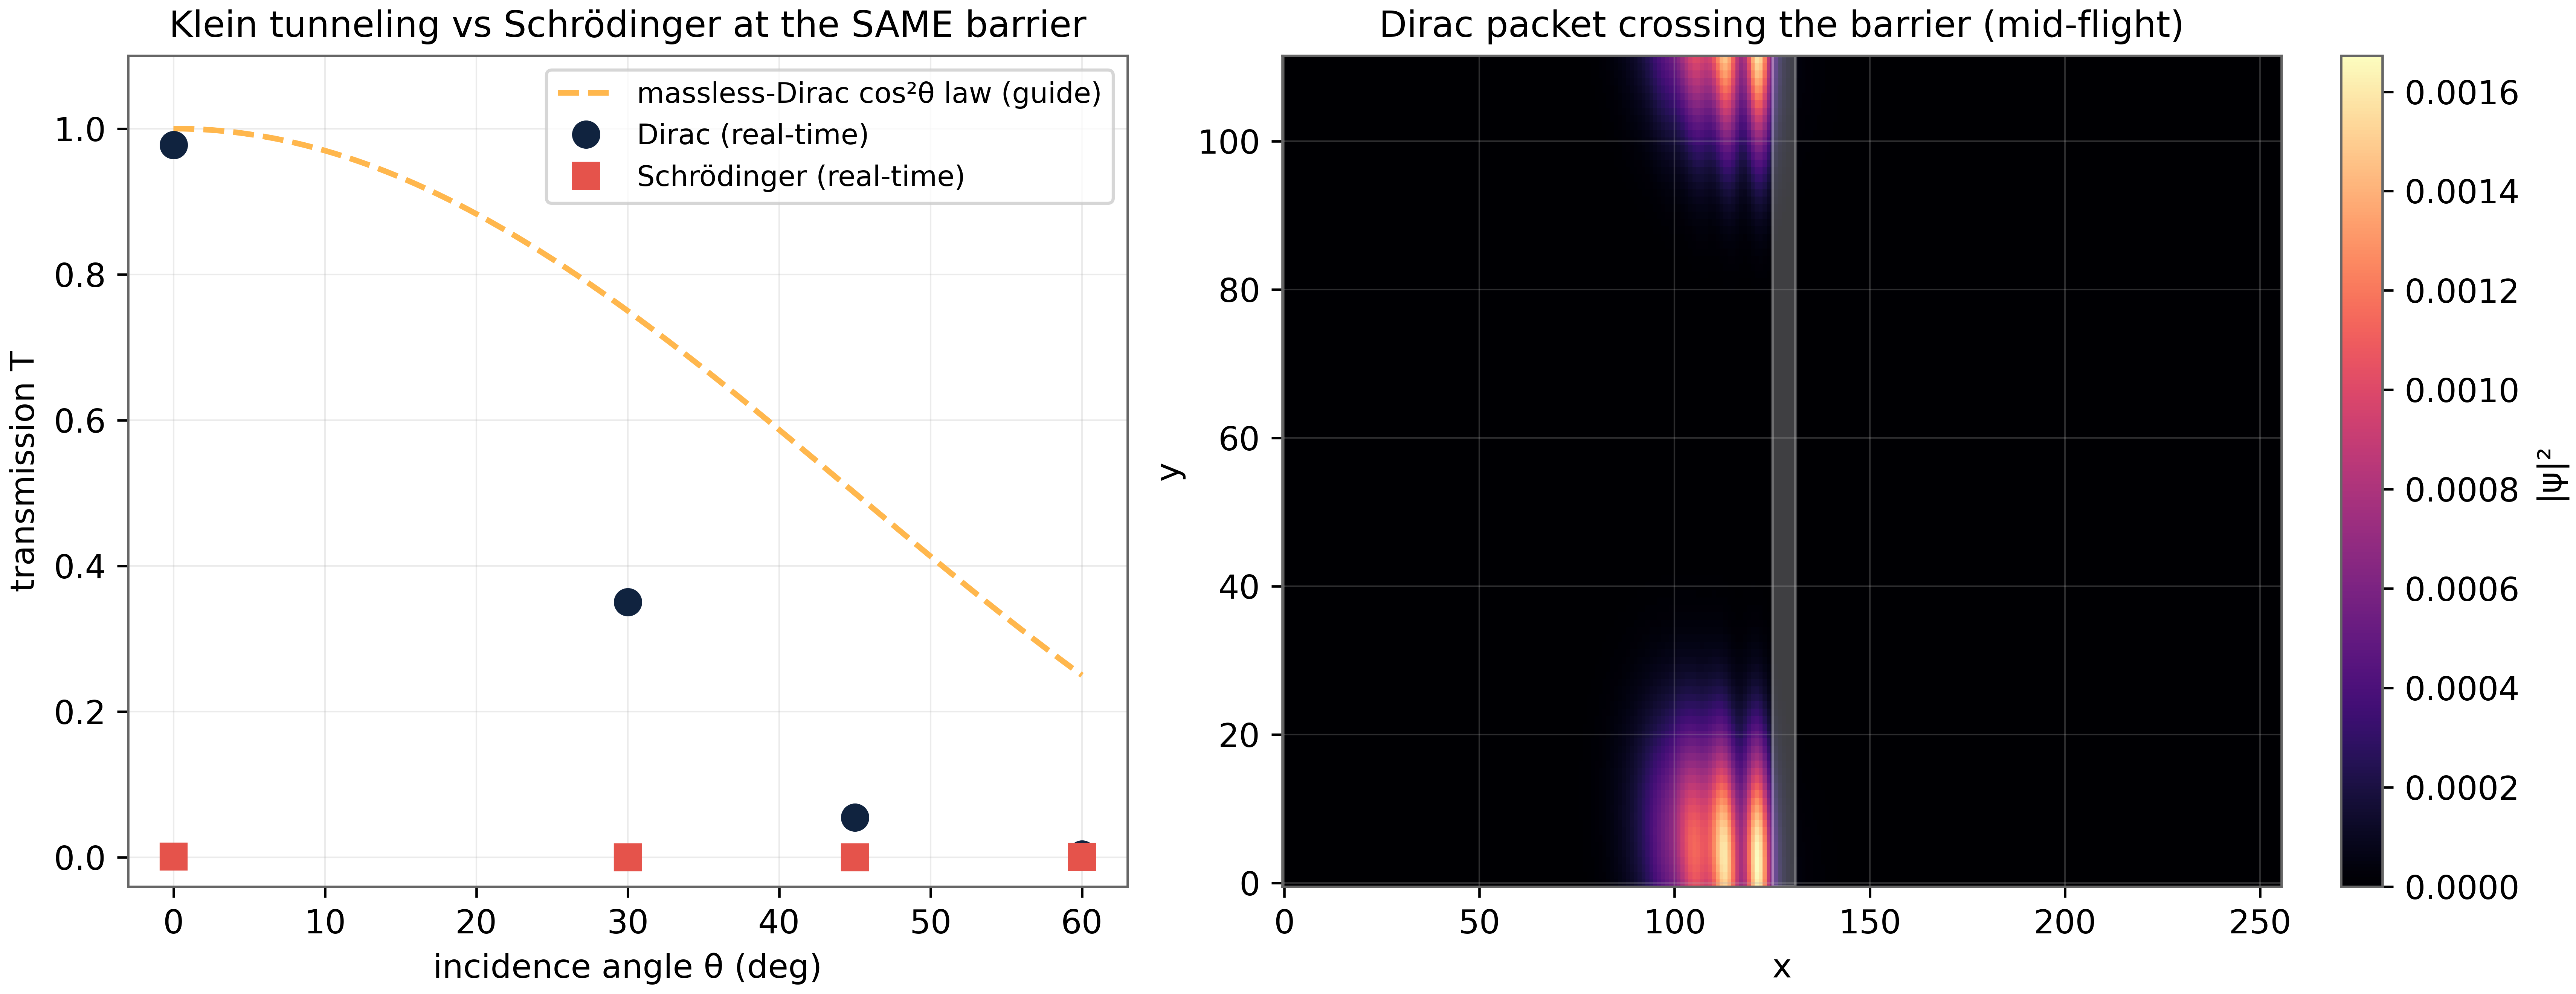
\includegraphics[max width=\columnwidth, max height=0.42\textheight]{figures/fig_D5_klein_tunneling.png}
\caption{Canonical D5 figure (600 dpi): transmission vs angle for both channels, produced by the original harness.}\label{fig:d5_1}
\end{figure}
\noindent\emph{Animation (played outside LaTeX): \texttt{figures/anim\_D5\_klein.gif}} --- Canonical animation: the Schrödinger packet failing to penetrate the barrier, frame by frame.\par\medskip
\begin{figure}[htbp]\centering
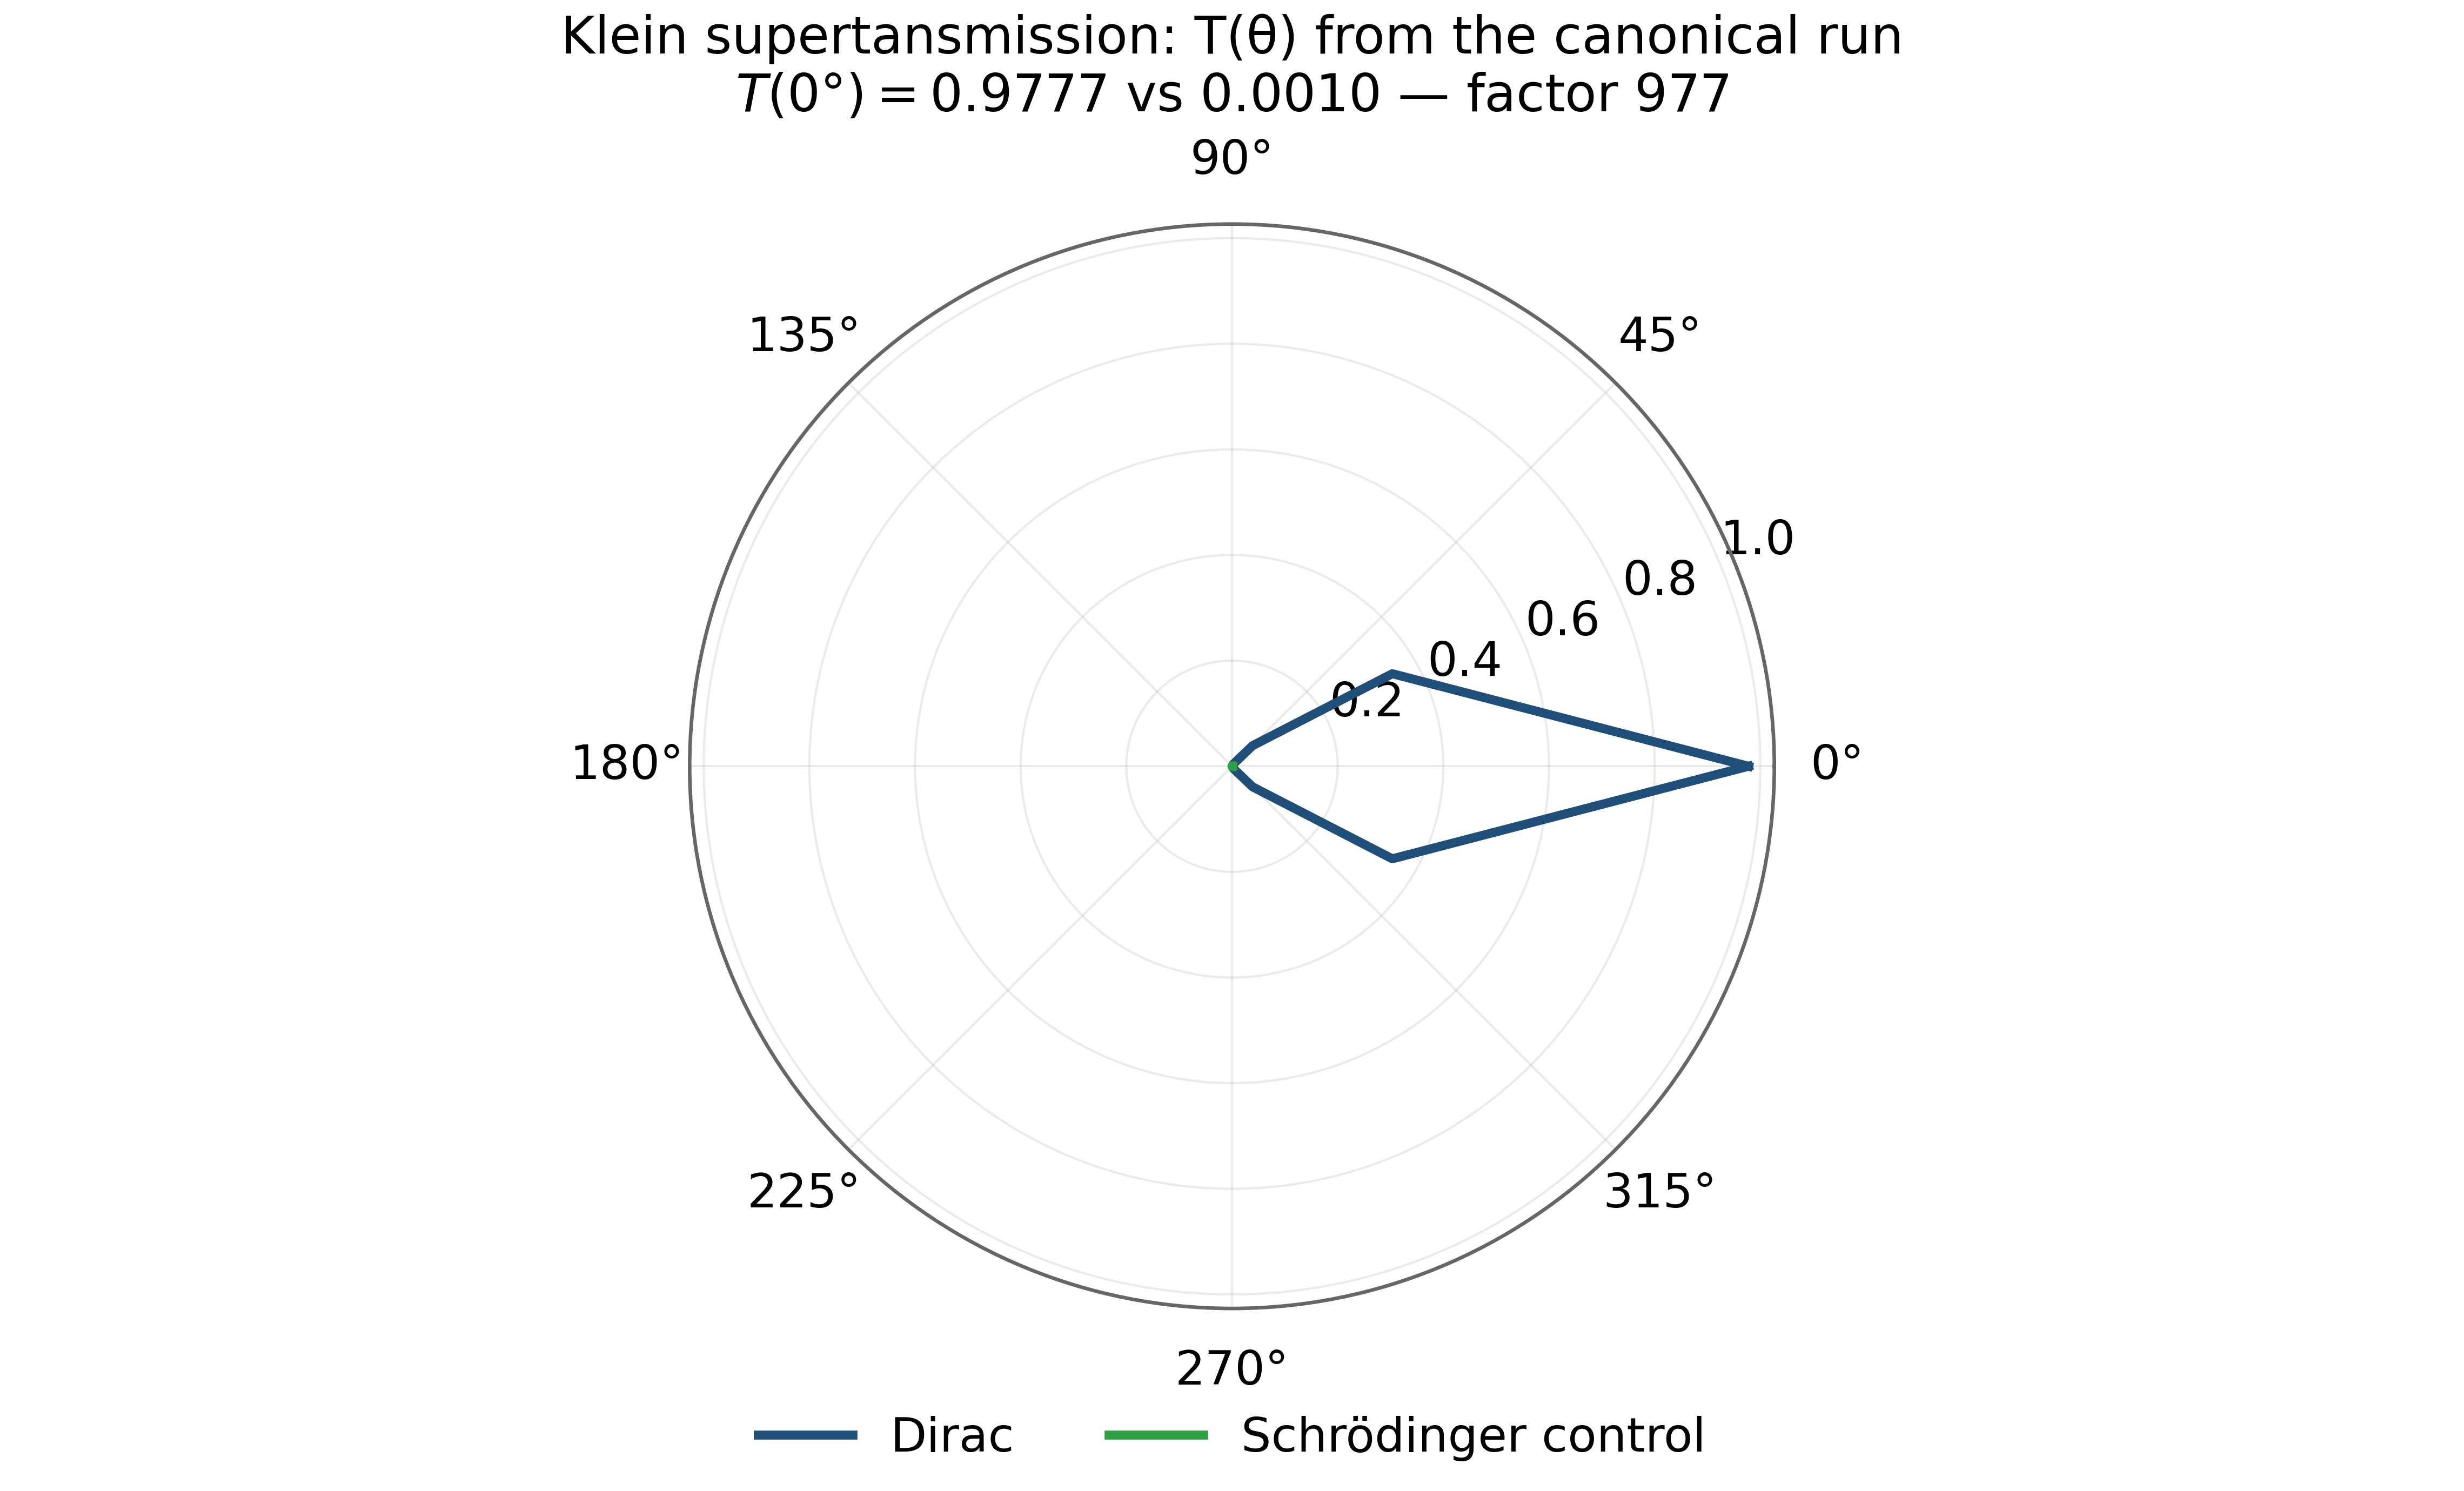
\includegraphics[max width=\columnwidth, max height=0.42\textheight]{figures/d05_extra_polar_transmission.png}
\caption{Companion polar diagram built from the canonical CSV: $T(\theta)$ for Dirac and Schrödinger channels; the Dirac lobe collapses with angle exactly as the pseudospin-mismatch law demands.}\label{fig:d5_3}
\end{figure}

\section{Discussion}
D5's two-channel design is the laboratory's template for honest dynamical claims: every striking number is paired with a control that would fail if the claim were an artifact. The factor of 977 is therefore not a benchmark to maximize but a mechanism to recognize -- and the mechanism, chirality, is exactly what the $\zeta$-decoration preserves in D8. That coherence is what licenses the transport tests on the decorated lattice.

For extensions, the natural upgrade is a Klein measurement on the full decorated operator with vortex scattering turned on, connecting D5 to D10's ensemble transport. The technical warning is documented in the monograph: packet statistics on small grids are sensitive to boundary wrap-around, so measurement windows must close before the first wrap -- the same discipline D10 uses.

\section{Reproducibility}
\begin{itemize}[leftmargin=1.2em, itemsep=0.15em]
\item \textbf{Single test:} \texttt{python3} \path{code/dirac_lab.py} \texttt{--test D5} (add \texttt{--quick} for a reduced pass; \texttt{--no-figures} to skip the 600-dpi figure).
\item \textbf{Canonical run:} \texttt{make all} regenerates the whole D1--D14 ledger into \path{results/}; this monograph's ledger is the verbatim per-check table of that run.
\item \textbf{Determinism:} seed 96 (parent convention); the $\zeta$ tables are the Odlyzko-derived files in \path{data/} with provenance in their headers.
\item \textbf{Figures:} the canonical figure was regenerated into this folder by the v1.4 harness (the original test function itself); companion panels are recomputed with the same modules (\path{scripts/make_extra_figures.py}). All figures are 600 dpi.
\item \textbf{Cross-verification:} Python-verified; the Julia cross-coverage map is \path{results/CROSS_VERIFICATION.md}.
\item \textbf{Artifacts in this folder:} \path{monograph.tex} (this document's source), \path{results.json} (machine-readable ledger), \path{figures/} (600-dpi figures), and the canonical CSV of the test.
\end{itemize}

\section*{References}
\begin{thebibliography}{99}\small
\bibitem{klein} O. Klein, Die Reflexion von Elektronen an einem Potentialsprung nach der relativistischen Dynamik von Dirac, Z. Phys. 53, 157 (1929).
\bibitem{dirac} P. A. M. Dirac, The quantum theory of the electron, Proc. R. Soc. A 117, 610 (1928).
\bibitem{parent} I. K. Isaev, AB-Cloud Research: the Hofstadter--Aharonov--Bohm realization of the Hilbert--P'olya programme (parent repository and test ledger), \url{https://github.com/wild8highlander/ab-cloud-research} (2026).
\end{thebibliography}

\vfill
\noindent\rule{\textwidth}{0.4pt}\\[0.2em]
{\footnotesize\color{labgray} AB-Cloud Dirac Laboratory · per-test monograph series v1.4 · compiled with Tectonic (LaTeX) · all numbers traceable to \texttt{results/run\_20261006\_full\_v13} · \texttt{D5} of 14.}

\end{document}